\subsection{Some useful relations}
\[(\bar{v}\gamma^\mu u)^*=\bar{u}\gamma^{\mu} v\]
any QED amplitute involving external fermions,when squared or summed over spin or overaged over spins, can be converted to trace of products of dirac metrics.for example for the process of figure \ref{fig:qedee} we have:\par
\begin{figure}
\begin{center}
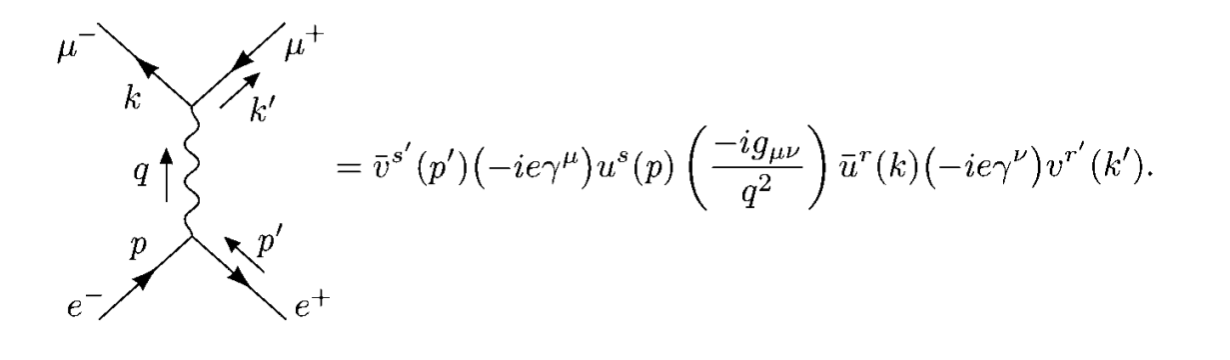
\includegraphics[height=5cm]{./figures/QEDee.PNG}
\caption{$e^+e^-\rightarrow \mu^+\mu^-$process}
\label{fig:qedee}
\end{center}
\end{figure}
\[\frac{1}{4}\sum_{spins}|\mathcal{M}|^2=\frac{e^4}{4q^4}trace[(\slashed{p'}-m_e)\gamma^\mu(\slashed{p'}+m_e)\gamma^\nu]trace[(\slashed{k}+m_\mu)\gamma_\mu(\slashed{k'}-m_\mu)\gamma_\nu]\]
the trace of an odd product of gamma metrics is zero(if n is odd):\par
\[trace[\gamma_1^{\mu}\cdots\gamma^{\mu'}_n]=0\]
\[tr[\gamma^\mu\gamma^\nu]=tr[2g^{\mu\nu}1-\gamma^\nu\gamma^\mu]\]
for the even number gamma metrics product ,we can anticommute the first one to the right and cycle it back ,we have the trace of two gamma metrics product:
\[tr[\gamma^\mu\gamma^\nu]=4g^{\mu\nu}\]
similarly for the four gamma metrics:\par
\[tr[\gamma^\mu\gamma^\nu\gamma^\rho\gamma^\sigma]=tr[2g^{\mu\nu}\gamma^\rho\gamma^\sigma-\gamma^\nu 2g^{\mu\rho}\gamma^\sigma+\gamma^\nu\gamma\rho 2g^{\mu\sigma}-\gamma^\nu\gamma^\rho\gamma^\sigma\gamma^\mu]\]
thus we have the following formula:
\[tr[\gamma^\mu\gamma^\nu\gamma^\rho\gamma^\sigma]=4(g^{\mu\nu}g^{\rho\sigma}-g^{\mu\rho}g^{\nu\sigma}+g^{\mu\sigma}g^{\nu\rho})\]
since $\gamma^5=i\gamma^0\gamma^1\gamma^2\gamma^3$,we have the trace fromula related to $\gamma^5$:
\[tr[\gamma^5]=0\]
\[tr[\gamma^\mu\gamma^\nu\gamma^5]=0\]
\[tr[\gamma^\mu\gamma^\nu\gamma^\rho\gamma^\sigma\gamma^5]=-4i\epsilon^{\mu\nu\rho\sigma}\]
and there are some formula for the antisymmetric tensor:
\[\epsilon^{\mu\nu\rho\sigma}\epsilon_{\mu\nu\rho\sigma}=-24\]
\[\epsilon^{\mu\nu\rho\sigma}\epsilon_{\mu\nu\rho\sigma'}=-6\delta^\sigma_{\sigma'}\]
\[\epsilon^{\alpha\beta\mu\nu}\epsilon_{\alpha\beta\rho\sigma}=-2(\delta^{\mu}_\rho\delta^\nu_\sigma-\delta^{\mu}_\sigma\delta^\nu_\rho)\]
and there is another useful formula:
\[tr[\gamma^\mu\gamma^\nu\gamma^\rho\gamma^\sigma\cdots]=tr[\cdots\gamma^\sigma\gamma^\rho\gamma^\nu\gamma^\mu]\]
if we set $C=\gamma^0\gamma^2$ then we have:
\[C^2=1\]
\[C\gamma^\mu C=-(\gamma^\mu)^T\]
when the gamma metrics is dotted inside the trace,one can always simplify it:
\[\gamma^\mu\gamma_\mu=g_{\mu\nu}\gamma^\mu\gamma^\nu=\frac{1}{2}g_{\mu\nu}\{\gamma^\mu,\gamma^\nu\}=g_{\mu\nu}g^{\mu\nu}=4\]
\[\gamma^\mu\gamma^\nu\gamma_\mu=-2\gamma^\nu\]
\[\gamma^\mu\gamma^\nu\gamma^\rho\gamma_\mu=4g^{\nu\rho}\]
\[\gamma^\mu\gamma^\nu\gamma^\rho\gamma^\sigma\gamma_\mu=-2\gamma^\sigma\gamma^\rho\gamma^\nu\]

\subsection{the unpolarized cross section for the process:$e^+e^-\rightarrow \mu^+\mu^-$}
when consider that $\frac{m_e}{m_{\mu}}$ is very small ,we can just set $m_e=0$,thus:
\[\frac{1}{4}\sum_{spins}|M|^2=\frac{8e^4}{q^4}[(p\bullet k)(p'\bullet k')+(p\bullet k')(p'\bullet k)+m_{\mu}^2(p\bullet p')]\]
after a long journey of calculation, we dervie the cross section for this process:
\[\frac{d\sigma}{d\Omega}=\frac{\alpha^2}{4E_{cm}^2}\sqrt{1-\frac{m_\mu ^2}{E^2}}[1+\frac{m_\mu ^2}{E^2}+(1-\frac{m_\mu ^2}{E^2})cos^2\theta]\]
and integrate it we can get the total cross section:
\[\sigma_{total}=\frac{4\pi \alpha^2}{3E_{cm}^2}\sqrt{1-\frac{m_\mu ^2}{E^2}}(1+\frac{1}{2}\frac{m_\mu ^2}{E^2})\]
we can define a unit of R:
\[R=\frac{4\pi \alpha^2}{3E_{cm}^2}\]
which means we regard  the cross section for the process $e^+e^-\rightarrow \mu^+\mu^-$ as a basic unit.\par

\subsection{$e^+e^-\rightarrow \mu^+\mu^-$:helicity structure}
\[\frac{d\sigma}{d\Omega}(e^-_Re^+_L\rightarrow \mu^-_L\mu^+_R)=\frac{\alpha^2}{4E_{cm}}(1+cos\theta)^2\]
\[\frac{d\sigma}{d\Omega}(e^-_Re^+_L\rightarrow \mu^-_R\mu^+_L)=\frac{\alpha^2}{4E_{cm}}(1-cos\theta)^2\]
\[\frac{d\sigma}{d\Omega}(e^-_Le^+_R\rightarrow \mu^-_L\mu^+_R)=\frac{\alpha^2}{4E_{cm}}(1-cos\theta)^2\]
\[\frac{d\sigma}{d\Omega}(e^-_Le^+_R\rightarrow \mu^-_R\mu^+_L)=\frac{\alpha^2}{4E_{cm}}(1+cos\theta)^2\]

for a right-hannded spinor ,we have:
\[\hat{p}\cdot\vec{\sigma}\eta=+\eta\]
for a left-handed spinor,we have:
\[\hat{p}\cdot\vec{\sigma}\eta=-\eta\]

some notes onn the bound state:
\[\sigma(e^+e^-\rightarrow B)=4\pi^2\frac{3\Gamma(B\rightarrow e^+e^-)}{M}\delta(E_{cm}^2-M^2)\]
the cross section for $e^+e^-$ to a bound state with spin-1 is that:
\[\sigma(e^+e^-\rightarrow B)=64\pi^3\alpha^2\frac{|\Psi(0)|^2}{M^3}\delta(E_{cm}^2-M^2)\]
and the decay rate  for the bound state is:
\[\Gamma(B\rightarrow e^+e^-)=\frac{16\pi\alpha^2}{3}\frac{|\Psi(0)|^2}{M^2}\]
\subsection{$e^-\mu^-\rightarrow e^-\mu^- $scatter}
the process's feymann diagram is presentend in figure \ref{fig:qedemu}.
\begin{figure}
\begin{center}
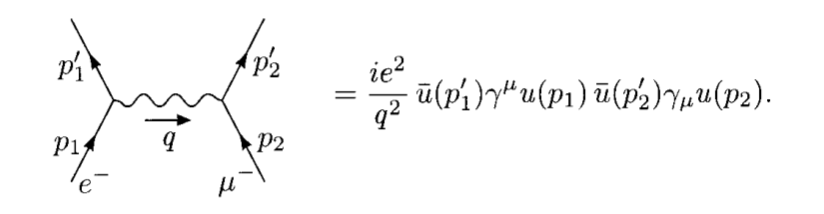
\includegraphics[height=5cm]{./figures/QEDemu.PNG}
\caption{$e^-\mu^-\rightarrow e^-\mu^-$process}
\label{fig:qedemu}
\end{center}
\end{figure}
just similar to the calculation with $e^+e^-\rightarrow \mu^+\mu^-$,we can easily get the deferiential cross section:
\[\frac{d\sigma}{d\Omega}=\frac{\alpha^2}{2k^2(E+k)^2(1-cos\theta)^2}[(E+k)^2+(E+kcos\theta)^2-m_{\mu}^2(1-cos\theta)]\]
Crossing Symmetry:
\[M(\phi(p)+\cdots\rightarrow\cdots)=M(\cdots\rightarrow \cdots\bar{\phi}(k))\]
where $\bar{phi}$ is the antipartical of $\phi$ and k=-p\par
Mandelstam Variable:
when the initial and final state are all two particals we can define the variables called Mandelstam Variable as below(see figure \ref{fig:man} for the process):
\begin{figure}
\begin{center}
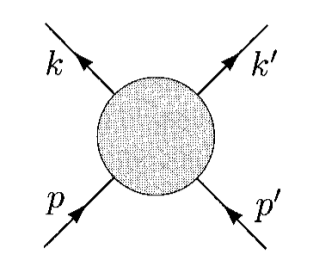
\includegraphics[height=5cm]{./figures/mandelstam.PNG}
\caption{illustration for the definition of mandelstam variable which involving 2-body to 2-body scattering process}
\label{fig:man}
\end{center}
\end{figure}
\[s=(p+p')^2=(k+k')^2\]
\[t=(k-p)^2=(k'-p')^2\]
\[u=(k'-p)^2=(k-p')^2\]
we can easily work out a relation:
\[s+t+u=\sum_i m_i^2\]

\subsection{Compton Scattering}
the feymann diagram for this process is presented in figure \ref{fig:compton}\par
\begin{figure}
\begin{center}
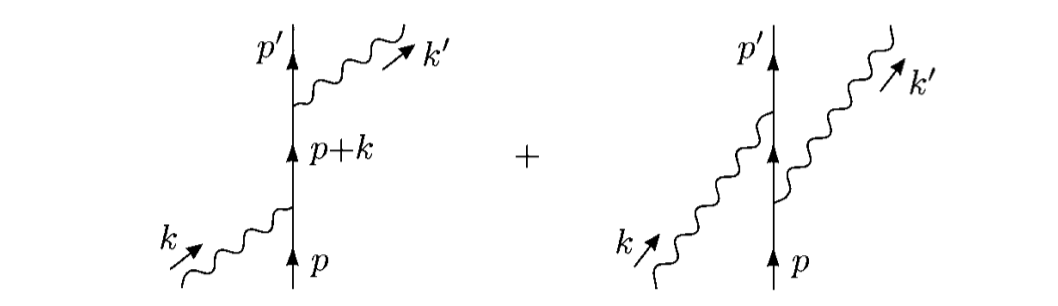
\includegraphics[height=5cm]{./figures/compton.PNG}
\caption{compton scattering process}
\label{fig:compton}
\end{center}
\end{figure}
so the amplitute is :
\[i\mathcal{M}=-ie^2\epsilon^*_\mu(k')\epsilon_\nu(k)\bar{u}(p')[\frac{\gamma^\mu\slashed{k}\gamma^\nu+2\gamma^{\mu}p^\nu}{2p\bullet k}+\frac{-\gamma^\nu\slashed{k'}\gamma^\mu+2\gamma^\nu p^\mu}{-2p\bullet k'}]u(p)\]

similar to the sum of electron polarization,there is also a good relation for sum of the photon polarization which is:
\[\sum_{polarization}\epsilon_\mu^*\epsilon_\nu\rightarrow -g_{\mu\nu}\]
with this in mind, we can easily get the quantity we want:
\[\frac{1}{4}\sum_{spins}|M|^2=\frac{e^4}{4}\{\frac{I}{(2p\bullet k)^2}+\frac{II}{(2p\bullet k)(2p\bullet k')}+\frac{III}{(2p\bullet k')(2p\bullet k)}+\frac{IIII}{(2p\bullet k')^2}\}\]

after a long journey of calculation we have the relations below:
\begin{align}
\notag I&=tr[(\slashed{p'}+m)(\gamma^\mu\slashed{k}\gamma^\nu+2\gamma^\mu p^\nu)(\slashed{p}+m)(\gamma_\nu\slashed{k}\gamma_\mu+2\gamma_\mu p_\nu)]\\
\notag&=16(4m^4-2m^2p\bullet p'+4m^2p\bullet k-2m^2p'\bullet k+2(p\bullet k)(p'\bullet k))\\
&=16(2m^4+m^2(s-m^2)-\frac{1}{2}(s-m^2)(u-m^2))
\end{align}
where the s,t,u is the Mandelstam Variables.\par
similarly we can work out the other three terms:
\begin{align}
IIII=16(2m^4+m^2(u-m^2)-\frac{1}{2}(s-m^2)(u-m^2))
\end{align}
\begin{align}
II=III=-8(4m^4+m^2(s-m^2)+m^2(u-m^2))
\end{align}
finally we have :
\[\frac{1}{4}\sum_{spins}|M|^2=2e^4[\frac{p\bullet k'}{p\bullet k}+\frac{p\bullet k}{p\bullet k'}+2m^2(\frac{1}{p\bullet k}-\frac{1}{p\bullet k'})+m^4(\frac{1}{p\bullet k}-\frac{1}{p\bullet k'})^2]\]
when we work in the fram of lab,we can make all the p,p',k,k'  illustrated as figure \ref{fig:compton2}. \par
\begin{figure}
\begin{center}
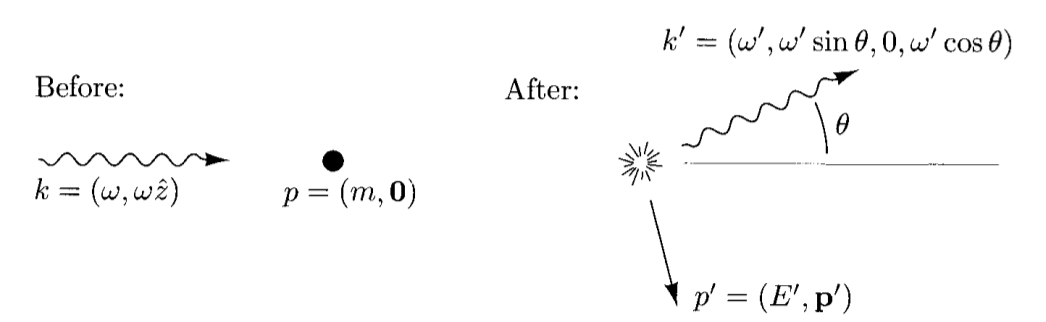
\includegraphics[height=5cm]{./figures/compton2.PNG}
\caption{compton scattering process in lab reference}
\label{fig:compton2}
\end{center}
\end{figure}
thus we have the differtial cross section:
\[\frac{d\sigma}{d(cos\theta)}=\frac{1}{2\omega}\frac{1}{2m}\frac{1}{8\pi}\frac{\omega'^2}{m\omega}(\frac{1}{4}\sum_{spins}|M|^2)\]
\[\frac{d\sigma}{d(cos\theta)}=\frac{\pi \alpha^2}{m^2}(\frac{\omega'}{\omega})^2[\frac{\omega'}{\omega}+\frac{\omega}{\omega'}-\sin ^2\theta]\]
where:
\[\omega'=\frac{\omega}{1+\frac{\omega}{m}(1-\cos\theta)}\]
this is called Klein-Nishina-Formula\par
when $\omega\rightarrow 0$,then $\frac{\omega'}{\omega}\rightarrow 0$,thus we have:
\[\frac{d\sigma}{d(cos\theta)}=\frac{\pi \alpha^2}{m^2}(1+\cos^2\theta)\]
which is the classical results which is known for all of us.\par


